
\chapter{Experimental Setup}\

This chapter explains the experimental setup built to run the simulations. First of all, the involved software are presented, then the specific files are described.\\
\begin{itemize}
\item{\textbf{Rhinoceros 3D\\}}
Rhino 3D is a stand-alone NURBS(Non Uniform Rational Basis-Splines)-based 3D modeling software. The software is commonly used for architecture, reverse engineering and graphic design.[3]

\item{\textbf{Grasshopper\\}}
Grasshopper 3D is a visual programming language running within Rhino. The principal advantage of this software is to parametrize the geometrics elements. It is an indispensable tool for modelling moving parts.

\item{\textbf{EnergyPlus\\}}
EnergyPlus is an energy analysis and thermal load simulation program. Based on a user's description of a building from the perspective of the building's physical make-up and associated mechanical and other systems, EnergyPlus calculates heating and cooling loads necessary to maintain thermal control set-points, conditions throughout a secondary HVAC (Heating, Ventilation and Air Conditioning) system and coil loads, and the energy consumption of primary plant equipment. Simultaneous integration of these -and many other- details verify that the EnergyPlus simulation performs as would the real building.[4]

\newpage

\item{\textbf{DIVA-Daylight Simulation\\}}
DIVA-for-Rhino is a highly optimized daylighting and energy modelling plug-in for the Rhinoceros - NURBS modeller. The plug-in was developed at the Graduate School of Design at Harvard University. DIVA-for-Rhino allows users to carry out a series of environmental performance evaluations of individual buildings  including Climate-Based Daylighting Metrics, Annual and Individual Time Step Glare Analysis, and Single Thermal Zone Energy and Load Calculations.
\end{itemize}

This softwares interacts to obtain a thermal simulation of our Adaptive Solar Facade equipped building. All static elements were designed in Rhinoceros (Section 2.1). Inside this model the moving parts, in our case the solar panels are added from Grasshopper.\\
DIVA is the connection between EnergyPlus and Rhinoceros, it extracts the input parameters from the Rhino model and inserts them in EnergyPlus. The user does not need to know EnergyPlus, because the Interface of DIVA provides all the necessary necessaries information.
The following sections describes the files designed to simulate the room which is equipped with the adaptive solar fa\c{c}ade.

\section{Room Description}
The analyzed room (Figure~\ref{room}) has an internal size of: 7 meters of length, 4.9 meters wide and 3.1 meters of height. The window has a 5 cm thick frame and a glass panel of 4.5 by 3 meters. The walls have a thickness of 15 cm.\\
The room has been drawn in Rhino as show in Figure~\ref{room}.
\begin{figure}[h]
 \centering
 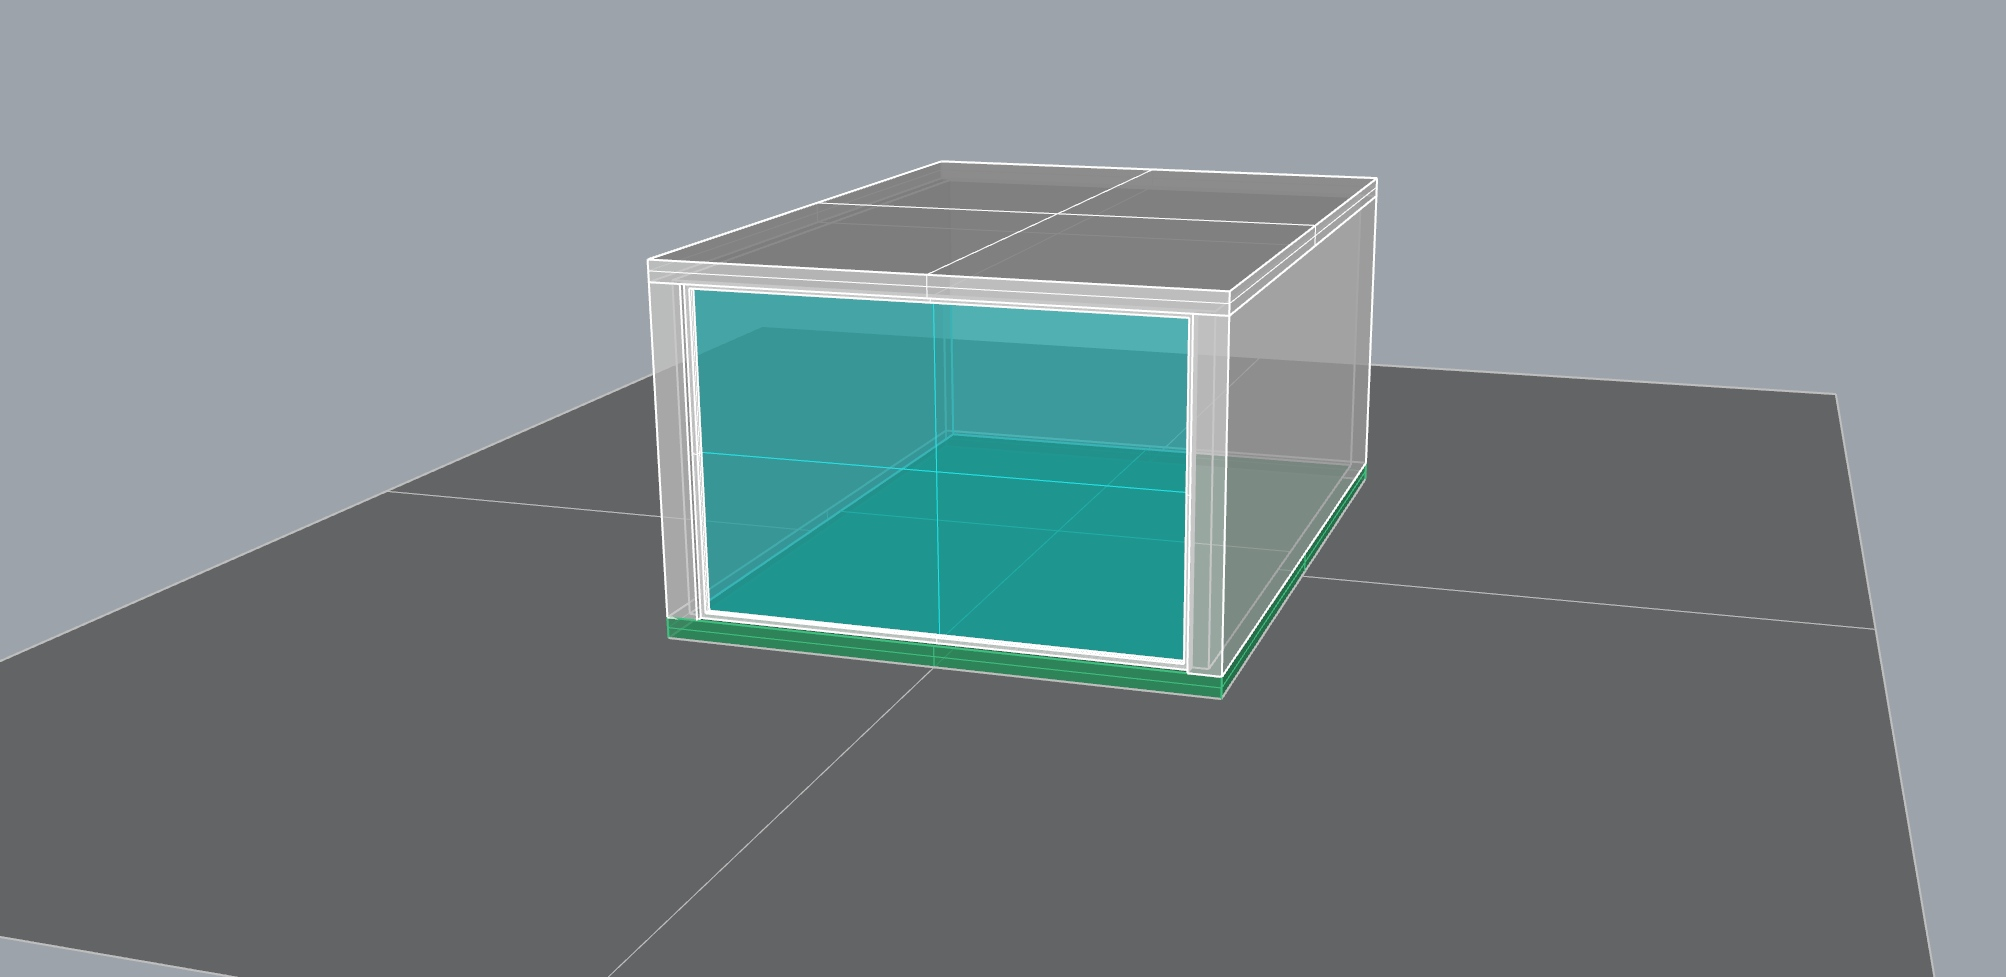
\includegraphics[width=140mm]{graphic/Room.jpg}
 \caption{Room}
 \label{room}
\end{figure}

\newpage
\section{Thermal Model}
The Rhino model (Section 2.1) doesn't have an influence in the simulations, but from this geometry the thermal model was build in Grasshopper (Figure~\ref{thermal_model}). \\

\begin{figure}[h]
 \centering
 \includegraphics[width=140mm]{graphic/Thermal_model.jpg}
 \caption{Thermal model}
 \label{thermal_model}
\end{figure}

\newpage

\section{Grasshopper program}

The Grasshopper program (Figure~\ref{GH_complete}) is structured with 3 groups of objects: the six bands in the middle corresponding to the six rows of solar panels, in the bubble frame on the left side all geometric elements common to all the solar panels have been grouped. These geometries have been adapted starting from a previous work of Andreas Thoma. The right side of the Grasshopper program is responsable for the simulations. These three groups are described below.

\subsection{Parametric design of a solar panel row}

The square solar panels have a side length of 400 mm and are extruded for 10 mm. The panels are rotated and displaced repeatedly to reach the desired position and orientation.\\

\begin{figure}[h]
 \centering
 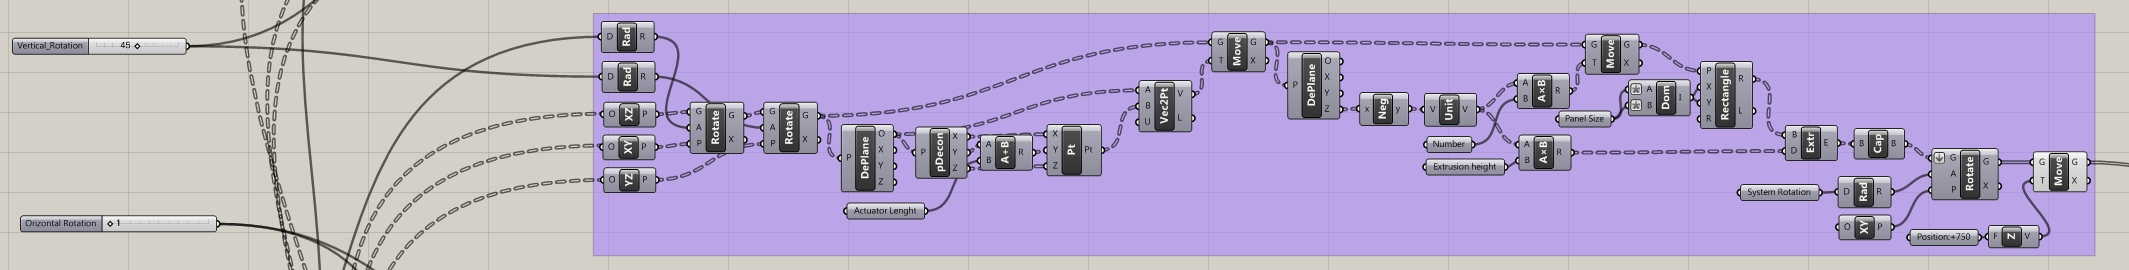
\includegraphics[width=150mm]{graphic/GH_panel.jpg}
 \caption{Single row of panels}
 \label{GH_panel}
\end{figure}

The six groups differs only for the inputs and for the position height on the facade. The top band is placed 1250 mm above the center. The center of the bands are spaced of 500 mm so that the bottom band  -1250 mm shifted.\\
A single slider controls the vertical rotation of all panels (upper left side in Figure~\ref{GH_panel}).
The horizontal rotation is controlled in groups of two rows of solar panels.

\subsection{Common geometrics elements}

The geometrical parameters common to all the rows of solar bands are have been grouped, these are: the grid angle (set to 0), the panel spacing (set to 500mm), and the frame size (set to 4500 mm in x-direction and 500 mm in y-direction).

\subsection{Thermal analysis}

The Thermal Analysis is performed by the Viper Component (Figure~\ref{GH_diva}). This element runs the DIVA environmental analysis program. The required inputs are:
\begin{itemize}
\item \textbf{Project Name:} connected to the vertical rotation slider to name the simulation file automatically
\item \textbf{Lighting Control:} threshold of 300 lux
\item \textbf{Zone:} the three internal walls, the ceiling and the floor are set as adiabatic. The external wall has an R-value of 13-7.5 $W / m^{2} K $
\item \textbf{Window:} Double glazing, glass 3mm/13mm capity fill with air
\item \textbf{Shade:} all the solar panels, with a Visible and a Solar Reflectance of 0.5
\item \textbf{Run:} connected to a toggle button
\end{itemize}

The chosen settings are:
\begin{itemize}
\item \textbf{Weather Location:} Geneva (the only available weather data for Switzerland)
\item \textbf{Occupancy:} Office (from 8 am to 6 pm)
\item \textbf{Simulation Parameters:} from 1 January to 31 December, 1 step per Hour.
\end{itemize}
And the chosen simulations output are:
\begin{itemize}
\item \textbf{IndoorTemp} Zone Mean Air Temperature [C]
\item \textbf{Heating E} Heating Energy Consumption (load divided by efficiency) [kWh]
\item \textbf{Cooling E} Cooling Energy Consumption (load divided by efficiency) [kWh]
\item \textbf{Elec: Light} Interior Lights: Electricity [kWh]
\end{itemize}

This is the setup for the programs used for the simulations of the next chapter.

\begin{figure}[h]
 \centering
 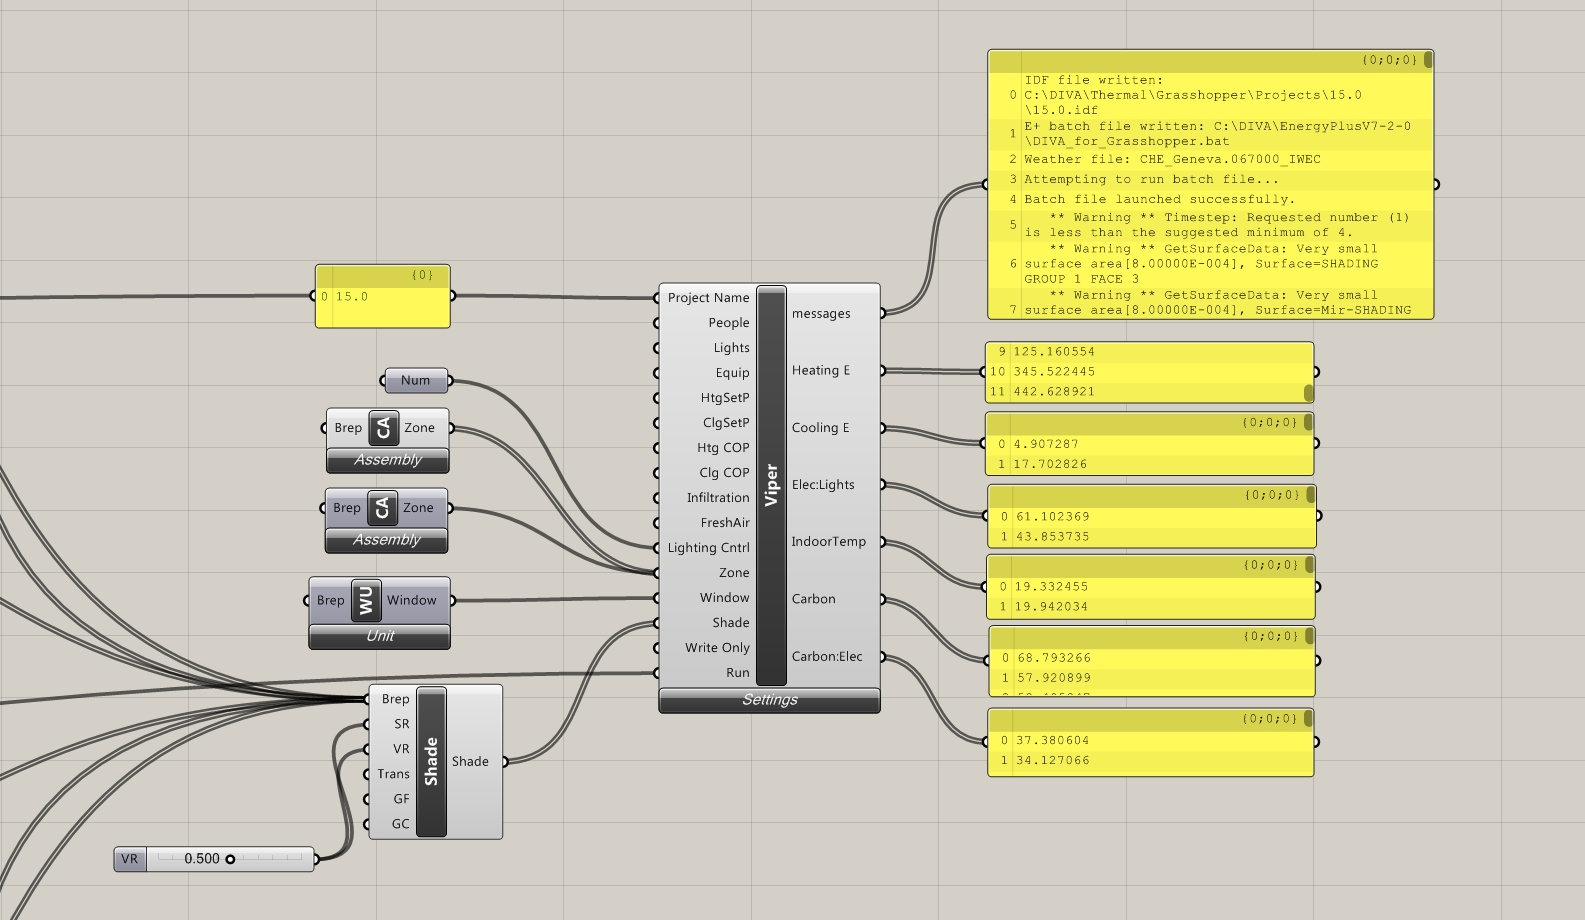
\includegraphics[width=140mm]{graphic/GH_diva.jpg}
 \caption{Viper Component}
 \label{GH_diva}
\end{figure}

\begin{figure}[h]
 \centering
 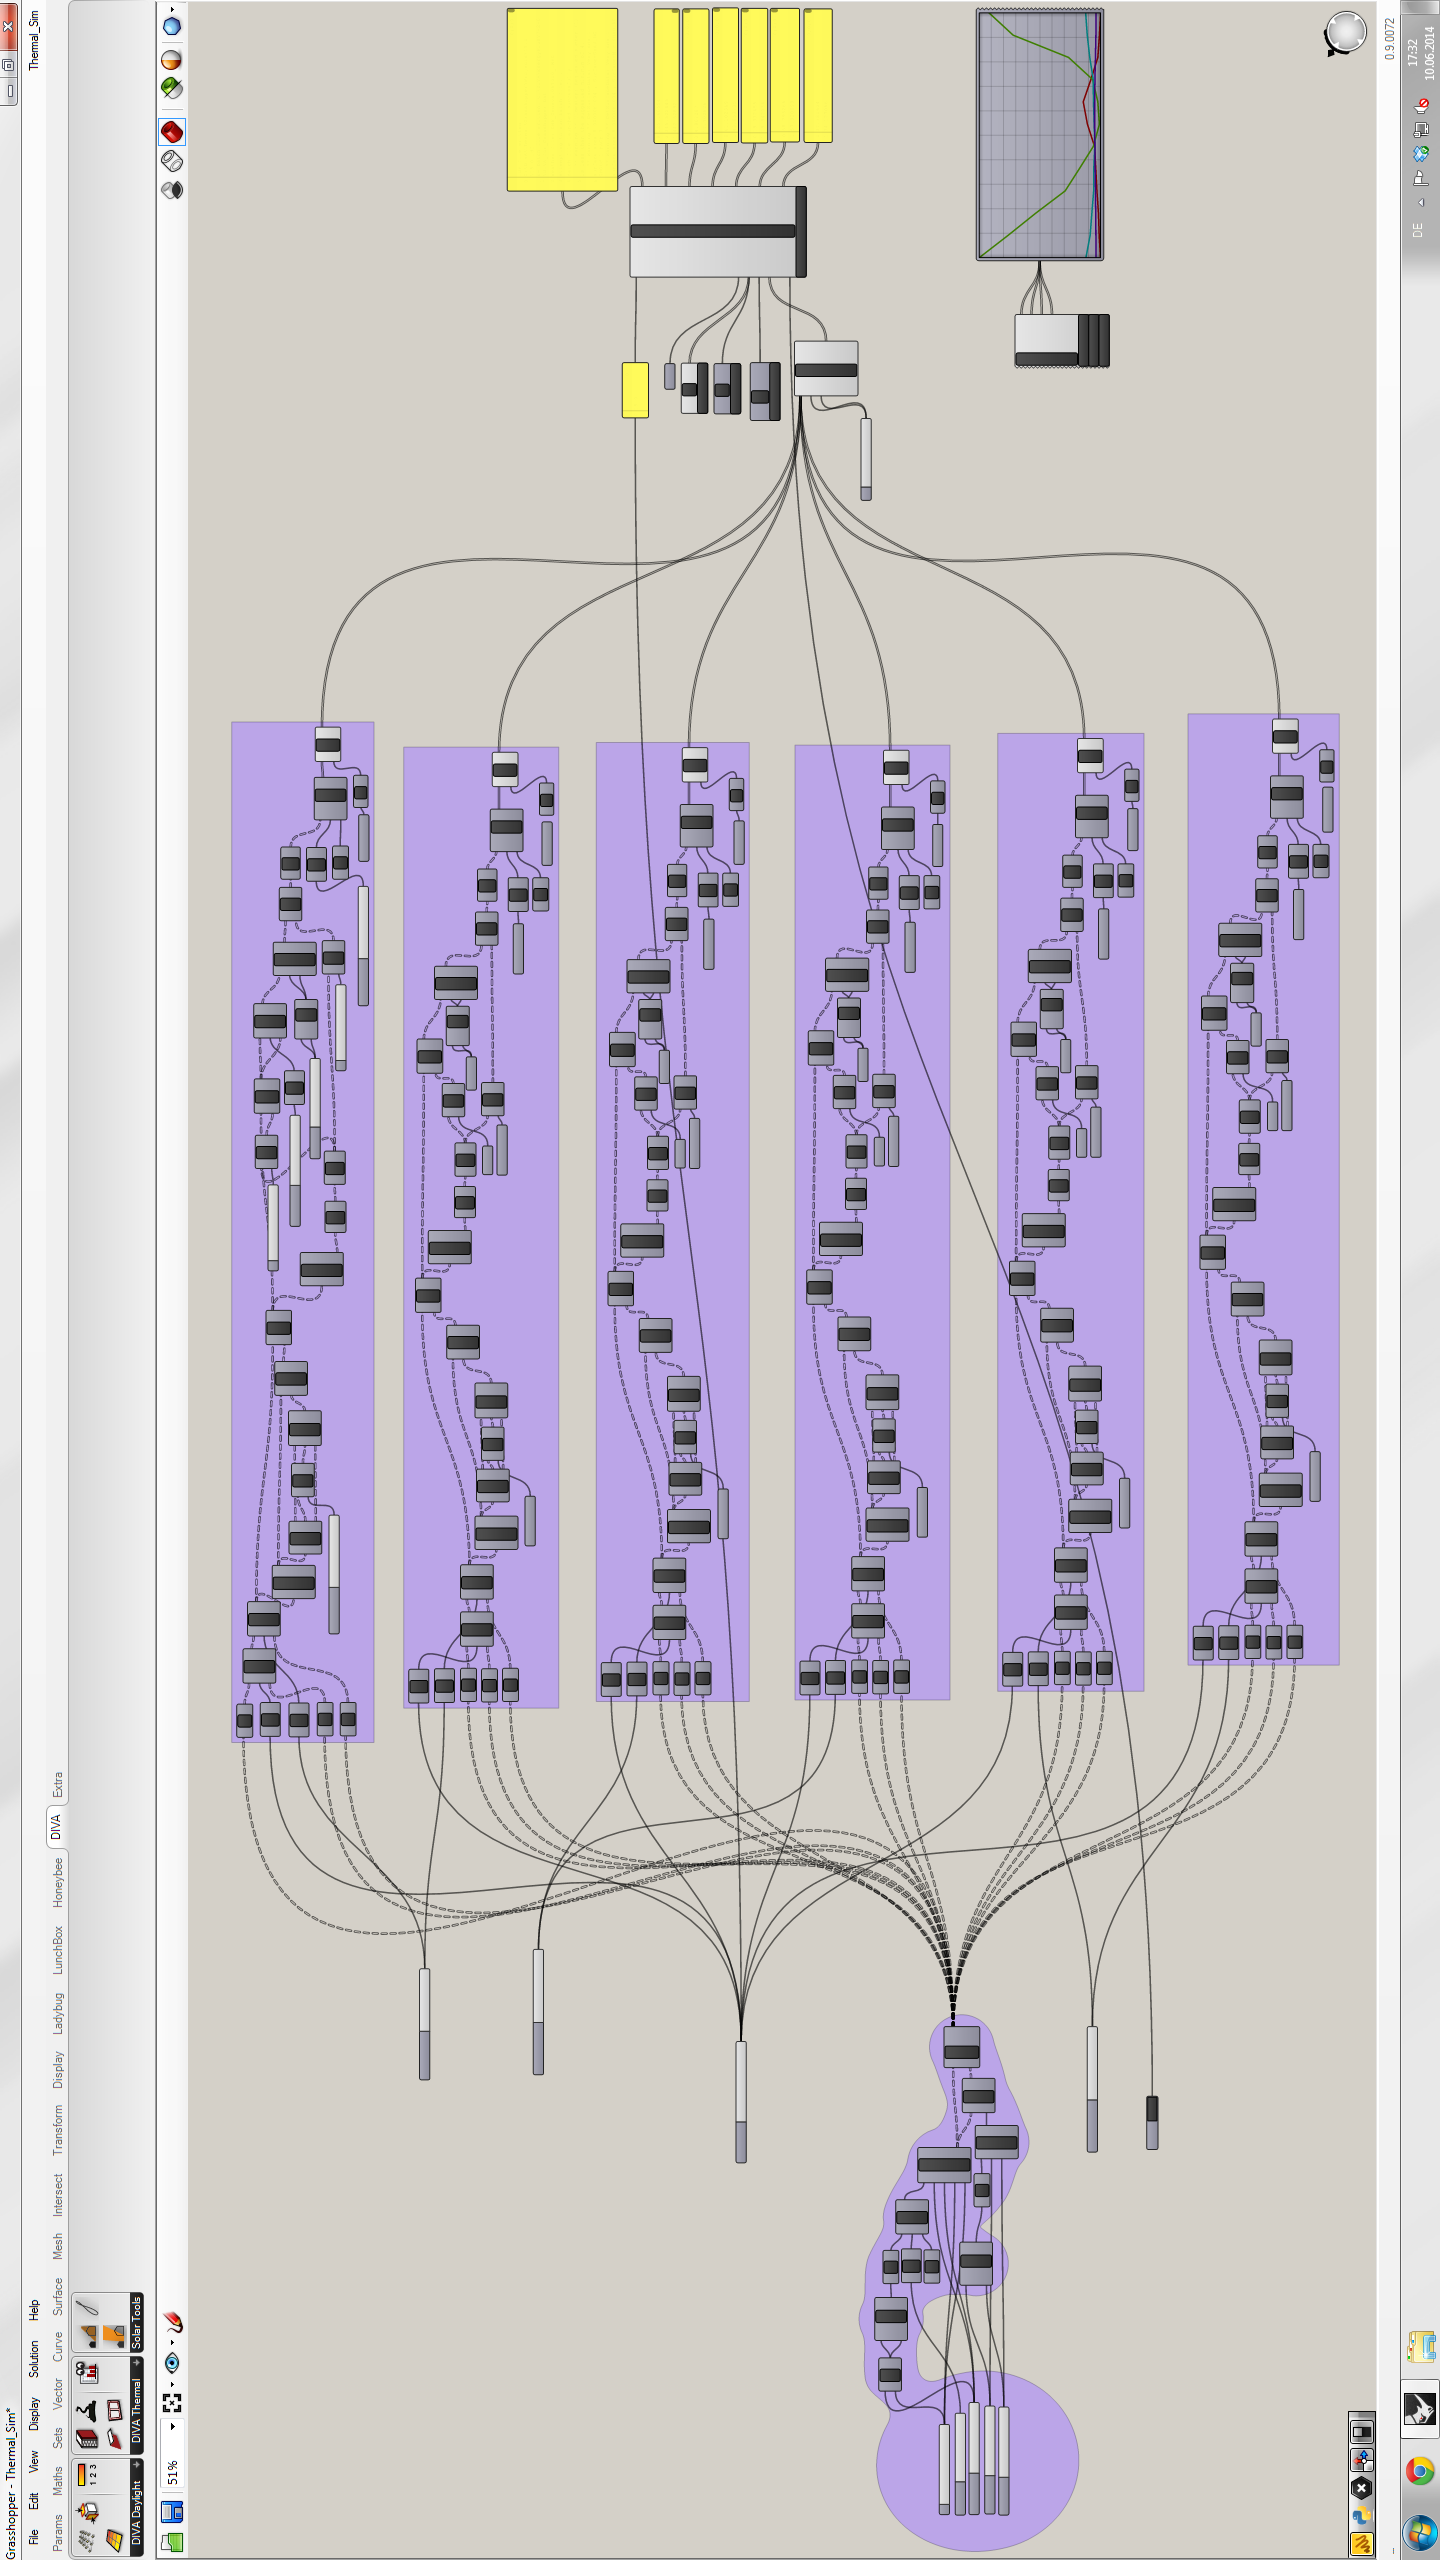
\includegraphics[width=130mm]{graphic/GH_complete.png}
 \caption{Grasshopper complete program}
 \label{GH_complete}
\end{figure}